%version of 03-02-20

\chapter{$\oplus \oplus$ Two Recurrence-Defined Number Families}
\label{ch:recurrent-numbers-appendix}


\noindent \fbox{\begin{minipage}{0.96\textwidth}
{\bf Topic-specific references}.

\smallskip

R.E.~Miller, N.~Pippenger, A.L.~Rosenberg, L.~Snyder (1979): Optimal 2,3-trees.  {\it SIAM J.~Comput.~8}, 42--59.

\smallskip

A.L.~Rosenberg (1979): Profile numbers.  {\it Fibonacci Quart.~17}(3), 259--264.

\smallskip

A.L.~Rosenberg and L.~Snyder (1978): Minimal-comparison 2,3-trees.  {\it SIAM J.~Comput.~7}, 465--480.

\end{minipage}
}

\bigskip

\noindent
This chapter is dedicated to two families of integers which share the recursively defined elegance of the Fibonacci numbers and the binomial coefficients.  The current two families do not share the level of elegance nor the range of application that the latter families do, but they can provide valuable experience dealing with recurrences that are a bit more complex than those that yield the Fibonacci numbers and the binomial coefficients.


\section{Lucas Numbers}
\label{sec:Lucas-numbers}
\index{Lucas numbers}
\index{Lucas sequence}

%version of 12-20-19

A continuing preoccupation of mathematicians is to understand why important mathematical structures exhibit their observed properties.  A common way to seek such understanding is to perturb the definition of a structure and study the effects of the perturbation.  While this stratagem leads to interesting, valuable results only sometimes, it is an invaluable tool in the hands of a gifted mathematician.  This section presents a brief survey of such a study by the 19th-century French mathematician Fran\c{c}ois Edouard Anatole Lucas (commonly known as Edouard Lucas).  \index{Lucas, Edouard}

\subsection{Definition}

\index{Fibonacci numbers!origin of name}
Lucas, who is credited with giving the name ``Fibonacci numbers'' to the sequence discovered by Leonardo Pisano, investigated the consequences of perturbing the initial conditions, $F(0) = F(1) = 1$, in the classical definition (\ref{eq:Fibonacci-defn}) of the Fibonacci sequence.

\medskip

Lucas's approach was simply to replace the Fibonacci sequence's initial values $\langle 1,1 \rangle$, with the values $\langle 2,1 \rangle$.  It turns out to be much more fruitful---in terms of more striking results and simpler proofs---to make a somewhat more drastic perturbation:

\smallskip

\index{Lucas sequence!definition}

The {\it Lucas sequence} is the infinite sequence of positive integers
\[ L(-1), \ L(0), \ L(1), \ L(2), \ldots \]
which is generated by the recurrence
\begin{eqnarray}
\nonumber
L(-1) & = & 2 \\
\label{eq:Lucas-defn-1}
L(0) & = & 1 \\
\nonumber
L(n) & = & L(n-1) \ + \ L(n-2) \ \ \ \mbox{ for all } n \geq 1
\end{eqnarray}
Because we conventionally index sequences by {\em nonnegative} numbers, we henceforth ignore $L(-1)$ and use the following {\em standard definition} of the Lucas sequence.
\begin{eqnarray}
\nonumber
L(0) & = & 1 \\
\label{eq:Lucas-defn-2}
L(1) & = & 3 \\
\nonumber
L(n) & = & L(n-1) \ + \ L(n-2) \ \ \ \mbox{ for all } n > 1
\end{eqnarray}

\medskip

The following finite sequences present the first few elements of both the Lucas sequence (for illustration) and the Fibonacci sequence (for comparison).
\[
\begin{array}{r|rrrrrrrrrrr}
n &
 0, & 1, & 2, & 3, &  4, &  5, &  6, &  7, &  8, &   9, & \ldots \\
\hline
L(n) &
 1, & 3, & 4, & 7, & 11, & 18, & 29, & 47, & 76, & 123, & \ldots \\
F(n) &
 1, & 1, & 2, & 3, &  5, &  8, & 13, & 21, & 34, &  55, & \ldots \\
\hline
\end{array}
\]

We begin our brief study of the Lucas sequence by noting that just a minor tweak converts the Fibonacci-related identity revealed in Proposition~\ref{thm:FiboSum-1} to an identity for Lucas numbers, as originally defined---beginning with $L(-1)$.

\begin{prop}
\label{thm:LucasSum-1}
For all integers $n \geq 0$,
\begin{equation}
\label{eq:multilinear-Lucas-1}
L(n+2) \ = \
1 \ + \ L(-1) \ + \ L(0) \ + \ L(1) \ + \ L(2) \ + \cdots + \ L(n)
\end{equation}
\end{prop}

\begin{proof}[Sketch]
We can literally repeat the proof of Proposition~\ref{thm:FiboSum-1}, with only a change in the induction's base case, which now becomes
\[ L(2) \ = \ L(-1) + L(0) + 1 \ = \ 2 + 1 + 1 \ = \ 4. \]
The body of the inductive argument holds for the Lucas sequence as well as for the Fibonacci sequence.  \qed
\end{proof}


\subsection{Relating the Lucas and Fibonacci Numbers}

\index{Ungerford, Margaret Wolfe}

There are several simple equations that relate the Lucas and Fibonacci numbers.  We present a few of the most aesthetically pleasing ones,\footnote{Aesthetically pleasing, that is, to the authors.  As noted by the author Margaret Wolfe Ungerford in {\it Molly Bawn} (1878), ``Beauty is in the eye of the beholder.''}~in terms of their exposing an intimate relationship between the two sequences.
\index{Fibonacci numbers!relations with Lucas numbers}
\index{Lucas numbers!relations with Fibonacci numbers}

\begin{prop}
\label{thm:Lucas-n:2Fibs}
For all $m, n \geq 1$
\begin{eqnarray}
\label{eq:L-F-a}
{\bf (a)} \  \hspace*{.49in}
L(n) & = & F(n+1) + F(n-1) \\
\label{eq:L-F-b}
{\bf (b)} \  \hspace*{.25in}
F(n+1) & = & \frac{1}{2} \big(F(n) \ + \ L(n) \big) \\
\label{eq:L-F-c}
{\bf (c)} \  
F(m + n-1) & = & \frac{1}{2} \big( F(m) \cdot L(n) \ + \ F(n) \cdot L(m) \big) \\
\label{eq:L-F-d}
{\bf (d)} \ \hspace*{.37in}
F(2n) & = & F(n) \cdot L(n)
\end{eqnarray}
\end{prop}

\begin{proof}
We consider the identities in turn.

\noindent {\bf (a)}
We proceed by induction.

\medskip

\noindent
{\sf Base case.}
Equation (\ref{eq:L-F-a}) holds when $n=1$ because
\[ L(1) = 3 = F(2) + F(0) = 2+1 \]

\medskip

\noindent
{\sf Inductive hypothesis}.
Assume that equation (\ref{eq:L-F-a}) holds for $L(2), L(3), \ldots, L(n)$.

\medskip

\noindent
{\sf Inductive extension}. 
Let us compute $L(n+1)$:
\begin{itemize}
\item
By definition (\ref{eq:Lucas-defn-2}),
\begin{equation}
\label{eq:L-FF-1}
L(n+1) \ = \ L(n) \ + \ L(n-1)
\end{equation}
\item
When we apply the inductive hypothesis to both addends in (\ref{eq:L-FF-1}), we obtain (after rearranging terms):
\begin{equation}
\label{eq:L-FF-2}
L(n+1) \ = \  F(n+1) \ + \ F(n) \ + \ F(n-1) \ + \ F(n-2)
\end{equation}
\item
Finally, we invoke the defining recurrence (\ref{eq:Fibonacci-defn}) of the Fibonacci numbers on the first two addends in (\ref{eq:L-FF-2}) and on the last two addends.  We thereby transform (\ref{eq:L-FF-2}) to equation (\ref{eq:L-F-a}), which validates the latter identity.
\end{itemize}

\bigskip

\noindent \fbox{
\begin{minipage}{0.95\textwidth}
{\bf Explanatory note}.

Notice that a proof similar to the preceding one yields the identity $L(n) = F(n+2) + F(n-2)$.  Similar, but more complicated, identities hold for larger arguments.  For the cases $n+3$ and $n+4$, for instance, one can establish the following pair of identities.
\begin{eqnarray}
\label{eq:LF:n+3}
L(n) & = & \frac{1}{2} (F(n+3)+F(n-3)) \\
\label{eq:LF:n+4}
L(n) & = & \frac{1}{3} (F(n+4)+F(n-4))
\end{eqnarray}
\end{minipage}
}
\bigskip

\noindent {\bf (b)}
By direct calculation, we derive the desired result:
\[ 2 F(n+1) \ = \ F(n+1) \ + \ F(n) \ + \ F(n-1) \ = \ L(n) \ + \ F(n)  \]

\bigskip

\noindent {\bf (c)}
This identity is verified via a somewhat complicated induction.  We fix parameter $n$ in the argument $F(m+n)$ and induce on parameter $m$.

\medskip

\noindent
{\sf Base case.}
Because $L(0) = F(0)= 1$, the instance $m=0$ of identity (\ref{eq:L-F-c}) reduces to identity (\ref{eq:L-F-b}), which we have just proved.  To wit,
\[ F(n+1) \ = \ \frac{1}{2} \big( L(n) \ + \ F(n) \big)
\ = \ \frac{1}{2} \big( F(0) \cdot L(n) \ + \ F(n) \cdot L(0) \big)
\]

\medskip 

\noindent
{\sf Inductive hypothesis}.
Let us assume that identity (\ref{eq:L-F-c}) holds for all $m \leq k$.

\ignore{\Denis Again, we should check for every proof the indices, the basic expressions are on $n$, fine.
The induction is on $m$ or $k$ up to $n$, and then, we derive for $n+1$...}

\medskip

\noindent
{\sf Inductive extension}.
Let us focus on instance $m = k+1$ of identity (\ref{eq:L-F-c}).  Note first that the classical Fibonacci recurrence (\ref{eq:Fibonacci-defn}) implies that
\[ F(n + k +1) \ = \ F(n + k) \ + \ F(n + k - 1). \]
When we apply the inductive hypothesis to both $F(n + k)$ and $F(n + k - 1)$, we obtain the following two identities.
\begin{eqnarray*}
F(n + k) & = & \frac{1}{2} \big( F(k-1) \cdot L(n) \ + \ F(n) \cdot L(k-1) \big) \\
F(n + k - 1) & = & \frac{1}{2} \big( F(k-2) \cdot L(n) \ + \ F(n) \cdot L(k-2) \big)
\end{eqnarray*}
Because both the Fibonacci and Lucas sequences obey the body of recurrence (\ref{eq:Fibonacci-defn}), the preceding equations combine to extend the induction.  To wit,
\begin{eqnarray*}
2 F(n + k +1) & = & 2 F(n + k) \ + \ 2 F(n + k - 1) \\
              & = & 
\big( F(k-1) \cdot L(n) \ + \ F(n) \cdot L(k-1) \big)
\ + \
\big( F(k-2) \cdot L(n) \ + \ F(n) \cdot L(k-2) \big) \\
              & = &
L(n) \cdot \big( F(k-1) \ + \ F(k-2) \big)
\ + \
F(n) \cdot \big( L(k-1) \ + \ L(k-2) \big) \\
              & = &
L(n) \cdot F(k) \ + \ F(n) \cdot L(k)
\end{eqnarray*}
The thus-extended induction verifies identity (\ref{eq:L-F-c}).

\bigskip

\noindent {\bf (d)}
Identity (\ref{eq:L-F-d}) is actually the case $m=n$ of identity (\ref{eq:L-F-c}).

\smallskip

This validates our final identity, which completes the proof.  \qed
\end{proof}




\section{Tree-Profile Numbers}
\label{sec:Tree-Profile-numbers}
\index{Tree-Profile numbers}

%version of 08-14-19


In the course of analyzing a genre of search tree called {\it
  2,3-trees},\footnote{These search trees are the lowest-index
  instances of the {\it B-trees} that have proved so useful in database
  implementations \cite{CLRS}.}~in \cite{MillerPRS79,RosenbergS78}, a
new number sequence was discovered.
\index{search trees}
\index{search trees!2,3-trees}
\index{search trees!B-trees}
Named {\it Tree-Profile numbers} \cite{Rosenberg79}, this family of
positive integers was found to be a close relative of the family of
binomial coefficients, both in its defining recurrence and in the
quite similar properties that the two families share.

\subsection{Definition}
\index{tree-profile numbers}

The {\it tree-profile numbers} are a doubly-indexed family
\[ \big\{ P(n,k) \big\}_{n \geq 1; \ k \geq 0}  \]
of positive integers specified by the following recursive definition.
\index{tree-profile numbers!definition}
\begin{equation}
\label{eq:TP-defn}
\begin{array}{ccl}
P(n,0) & \equiv & 1 \ \ \ \ \ \mbox{ for all } \ n \geq 1 \\
  & & \\
P(n,1) & = &
  {\displaystyle
\left\{
\begin{array}{cl}
 1 & \mbox{ for } \ n=1 \\
 2 & \mbox{ for all } \ n > 1
\end{array}
\right.  } \\
  & & \\
P(n+1, k+1) & = & P(n,k) + 2 P(n, k-1) \ \ \  \mbox{ for all } n > 1, k > 0
\end{array}
\end{equation}
\index{tree-profile numbers!triangle of numbers}

This somewhat complicated definition can be better understood with the
help of an analogue of Pascal's Triangle that we call the {\it
  Tree-profile Triangle}.  The reader may want to compare
Fig.~\ref{fig:pascal-triangle} with Fig.~\ref{fig:TP-triangle}.

\begin{figure}[htb]
\[
\begin{array}{c||r|r|r|r|r|r|r|r|r|r|r}
P(n, k) & k=0 & k=1 & k=2 & k=3 & k=4 & k=5 & k=6 & k=7 & k=8 & k=9 & \ldots \\
\hline
\hline
n=1 &  1 &  1 &    &    &     &     &     &     &     &     \\
\hline
n=2 &  1 &  2 &  3 &  2 &     &     &     &     &     &     \\
\hline
n=3 &  1 &  2 &  4 &  7 &   8 &   4 &     &     &     &     \\
\hline
n=4 &  1 &  2 &  4 &  8 &  15 &  22 &  20 &   8 &     &     \\
\hline
n=5 &  1 &  2 &  4 &  8 &  16 &  31 &  52 &  64 & 48  &  16 \\
\hline
n=6 &  1 &  2 &  4 &  8 &  16 &  32 &  63 & 114 & 168 & 176 \\
\hline
n=7 &  1 &  2 &  4 &  8 &  16 &  32 &  64 & 127 & 240 & 396 \\
\hline
n=8 &  1 &  2 &  4 &  8 &  16 &  32 &  64 & 128 & 255 & 494 \\
\hline
n=9 &  1 &  2 &  4 &  8 &  16 &  32 &  64 & 128 & 256 & 511 \\
\hline
\vdots &\vdots &\vdots &\vdots &\vdots &\vdots &\vdots &\vdots &\vdots
&\vdots &\vdots &\ddots
\end{array}
\] 
\caption{A ``prefix'' of the Tree-Profile Triangle, for $n,k \leq 9$.}
\label{fig:TP-triangle}
\end{figure}


\subsection{Triangle-Profile numbers and binomial coefficients}
\index{tree-profile numbers!relations with binomial coefficients}

\begin{prop}
\label{thm:TP=sum-of-bincoeff}
For all $n \geq 1$ and all $k \geq 0$,
\begin{equation}
\label{eq:TP=sum-of-bincoeff}
P(n,k) \ = \ 2^{k-n} \cdot \sum_{i=0}^{2n-k} {n \choose i}
\end{equation}
\end{prop}

\begin{proof}
We proceed by induction on $n$.

\medskip

\noindent
{\it The base case.}
The case $n=1$ of (\ref{eq:TP=sum-of-bincoeff}) follows from the
``boundary cases'' of definition (\ref{eq:TP-defn}).

\medskip

\ignore{\Denis same remark as before about the indices...}

\noindent
{\it The inductive hypothesis.}
Let us assume that (\ref{eq:TP=sum-of-bincoeff}) holds for all $n$ up
to (but not including) some integer $m$.  Focus on an arbitrary
Tree-Profile number $P(m,k)$.
\begin{itemize}
\item
If $k \in \{0,1\}$, then the ``boundary cases'' of definition
(\ref{eq:TP-defn}) assure us that
\[
P(m,k) \ \ = \ \ 2^k \ \ = \ \ 2^{k-n} \cdot 2^n \ \ = \ \ 
2^{k-n} \cdot \sum_{i=0}^{2n-k} {n \choose i}
\]

\item
If $k > 1$, then the defining recurrence in (\ref{eq:TP-defn})
combines with the inductive hypothesis to yield:
\begin{eqnarray*}
\nonumber
P(m, k) & = &
   P(m-1, k-1) \ + \ 2 P(m-1, k-2) \\
        & = &
   2^{k-m} \cdot \sum_{i=0}^{2m-k-2} {m-1 \choose i}
   \ + \
   2^{k-m} \cdot \sum_{j=0}^{2m-k-1} {m-1 \choose i} \\
        & = &
   2^{k-m} \cdot {m \choose 0}
   \ + \
   2^{k-m} \cdot \sum_{i=1}^{2m-k-1} {m-1 \choose i}
   \ + \
   {{m-1} \choose {i-1}} \\
        & = &
   2^{k-m} \cdot \sum_{i=0}^{2m-k-1} {m \choose i}.
\end{eqnarray*}
\end{itemize}
The induction is thus extended, thereby establishing the proposition.
\qed
\end{proof}

Proposition~\ref{thm:TP=sum-of-bincoeff} explains the proliferation of
powers of $2$ in the Tree-Profile Triangle.

\begin{corol}
For all $n > k$, $P(n,k) = 2^k$.
\end{corol}

\medskip

Finally, we derive the successor Tree-Profile values that allow us to
generate the Tree-Profile Triangle.

\begin{prop}
\label{thm:successor-TP-values}
\begin{eqnarray*}
\nonumber
\mathbf{(a)} \ \
P(n, k+1) & = & 
  2 P(n,k) - 2^{k-n+1} {n \choose {k-n+1}} \\
\label{eq:successor-TP-values}
          &   & \\
\nonumber
\mathbf{(b)} \ \
P(n+1, k) & = &
  P(n,k) + 2^{k-n-1} \left[ {n \choose {k-n}} + {{n+1} \choose {k-n}} \right]
\end{eqnarray*}
\end{prop}

\begin{proof}
The major recurrence in (\ref{eq:TP-defn}) can be decomposed into the
following triplet of recurrences.
\begin{eqnarray}
\label{eq:TP-recurrence-1}
P(n, k)   & = & P(n-1, k-1) \ + \ 2 P(n-1, k-2) \\
\label{eq:TP-recurrence-2}
P(n, k+1) & = & P(n-1, k) \ + \ 2 P(n-1, k-1) \\
\label{eq:TP-recurrence-3}
P(n+1, k) & = & P(n, k-1) \ + \ 2 P(n, k-2)
\end{eqnarray}
We use the recurrences in this triplet to attack the two alleged
recurrences in the proposition.
\medskip

\noindent {\bf (a)}
Combining recurrences (\ref{eq:TP-recurrence-1}) and
(\ref{eq:TP-recurrence-2}) leads, via
Proposition~\ref{thm:TP=sum-of-bincoeff}, to the following chain of
equalities\footnote{Nothing magical here! The idea to combine $P(n, k+1)$ and $-2 P(n, k)$
is for removing the common term $P(n-1, k-1)$}.
\begin{eqnarray*}
P(n, k+1) \ - \ 2 \ P(n, k)
  & = &
P(n-1, k) \ - \ 4 P(n-1, k-2) \\
  & = &
2^{k-n+1} \cdot \left[
\sum_{i=0}^{2n-k-3} {{n-1} \choose i} \ - \
\sum_{i=0}^{2n-k-1} {{n-1} \choose i}
\right] \\
  & = & 
- 2^{k-n+1} \cdot \left[
{{n-1} \choose {2n-k-2}} \ + \ {{n-1} \choose {2n-k-1}}
\right] \\
  & = &
- 2^{k-n+1} \cdot {n \choose k-n+1}.
\end{eqnarray*}
This chain thus yields part {\bf (a)} of the proposition.

\medskip

\noindent {\bf (b)}
This part of the proposition follows by direct calculation from
recurrence (\ref{eq:TP-recurrence-3}) and
Proposition~\ref{thm:TP=sum-of-bincoeff}.  To wit,
\begin{eqnarray*}
P(n+1, k) \ - \ P(n, k)
  & = &
P(n, k-1) \ + \ 2 P(n, k-2) \ - \ P(n,k) \\
  & = &
2^{k-n-1} \cdot \left[
\sum_{i=0}^{2n-k+1} {n \choose i}
 \ - \ \sum_{i=0}^{2n-k+2} {n \choose i}
 \ - \ 2 \sum_{i=0}^{2n-k} {n \choose i}
\right] \\
  & = & 
2^{k-n-1} \cdot \left[
  2 {n \choose {2n-k}} \ + \ {n \choose {2n-k+1}} \right] \\
  & = &
2^{k-n-1} \cdot \left[
   {n \choose {k-n}} \ + \ {{n+1} \choose {k-n}} \right]
\end{eqnarray*}
This chain thus yields part {\bf (b)} of the proposition, completing
the proof.
\qed
\end{proof}

\subsection{The summation formula for Triangle-Profile numbers}
\index{tree-profile numbers!summation formula}

We observed in Proposition~\ref{thm:sumsof-binomcoeff} that the
binomial coefficients in successive rows of Pascal's Triangle sum to
successive powers of $2$.  While not quite matching that level of
elegance, we show now that the Tree-Profile numbers in successive rows
of the Tree-Profile Triangle sum to $1$ less than successive powers of
$3$.

\begin{prop}
\label{thm:TP-summation}
For all $n \in \N^+$,
\begin{equation}
\label{eq:TP-summation}
S_n \ \ \eqdef \ \ \sum_{k=0}^{2n-1} P(n,k) \ \ = \ \ 3^n -1.
\end{equation}
\end{prop}
 
\begin{proof}
We begin with the following consequence of
Proposition~\ref{thm:TP=sum-of-bincoeff}:
\[
S(n) \ \ = \ \
  \sum_{k=0}^{2n-1} P(n,k)
     \ \ = \ \
  1 \ + \ \sum_{k=0}^{2n-1} P(n,k+1).
\]
If we now invoke Proposition~\ref{thm:successor-TP-values}(a), then we
find that
\[
S(n) \ \ = \ \ 1 \ + \ 2 \cdot \sum_{k=0}^{2n-1} 
  \big( P(n,k) \ - \ 2^{k-n} {n \choose {k-n+1}} \big).
\]

We can combine the preceding expressions with the ``restricted''
Binomial Theorem (Theorem~\ref{thm:restricted-binomial-thm}) to
generate the following chain of equalities.

{\Denis The first equality is not straightforward, I think an intermediate step is needed here...}
\begin{eqnarray*}
S(n) & = & 
\sum_{j=0}^{2n-1} 2^{n-j} {n \choose j} \ - \ 1  \\
     & = &
2^n \cdot \sum_{j=0}^{2n-1} 2^{-j} {n \choose j} \ - \ 1 \\
     & = & 
2^n \cdot (3/2)^n \ - \ 1 \\
     & = &
3^n -1.
\end{eqnarray*}

The summation formula (\ref{eq:TP-summation}) follows.
\qed
\end{proof}

{\Denis I draw a picture similarly as for the Pascal's triangle, let think where and how to put it in the text...}
\begin{figure}
\begin{center}
        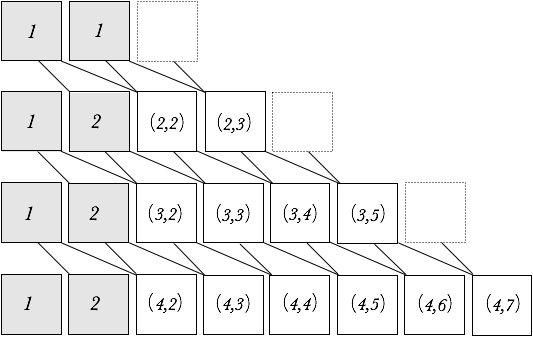
\includegraphics[scale=0.4]{FiguresMaths/TreeProfile}
        \caption{Graphical construction of the triangle profile numbers.}
        \label{Fig:treeprofile}
\end{center}
\end{figure}



